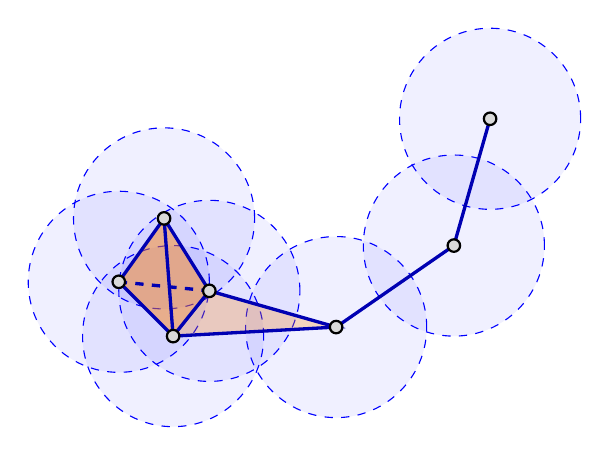
\begin{tikzpicture}[scale=1.15, font=\small,
  vtx/.style={circle, draw=black, fill=gray!30, thick, inner sep=1.6pt}]
% centres of seven open discs of radius 1
\coordinate (a) at (0,0.9);
\coordinate (b) at (-0.5,0.2);
\coordinate (c) at (0.1,-0.4);
\coordinate (d) at (0.5,0.1);
\coordinate (e) at (1.9,-0.3);
\coordinate (f) at (3.2,0.6);
\coordinate (g) at (3.6,2.0);
% the discs U_i
\foreach \p in {a,b,c,d,e,f,g}
  \draw[blue, dashed, fill=blue, fill opacity=0.06] (\p) circle (1);
% the nerve: a solid tetrahedron abcd, a triangle cde, edges ef and fg
\fill[orange, opacity=0.45] (a) -- (b) -- (c) -- (d) -- cycle;
\fill[orange, opacity=0.25] (c) -- (d) -- (e) -- cycle;
\draw[very thick, blue!70!black] (a) -- (b) -- (c) -- (d) -- cycle (a) -- (c);
\draw[very thick, blue!70!black, dashed] (b) -- (d);
\draw[very thick, blue!70!black] (c) -- (e) -- (d);
\draw[very thick, blue!70!black] (e) -- (f) -- (g);
\foreach \p in {a,b,c,d,e,f,g} \node[vtx] at (\p) {};
\end{tikzpicture}
